%% This is an example first chapter.  You should put chapter/appendix that you
%% write into a separate file, and add a line \include{yourfilename} to
%% main.tex, where `yourfilename.tex' is the name of the chapter/appendix file.
%% You can process specific files by typing their names in at the
%% \files=
%% prompt when you run the file main.tex through LaTeX.
\chapter{Introduction}

Speech is most important medium of conveying opinions and expressing feeling and thoughts.
Human convert their thought into speech by using words, phrases and sentences in order to communicate with each other \cite{mumtaz2016break}. Speech is produced when air is exhaled by the lungs and vibrations are produced by air, these vibrations got a proper waveform shape by glottal cords and vocal tract. Text to Speech synthesis is the process of conversion of raw text into speech signals. It works by concatenation of small segments of recorded speech called phonemes \cite{khilari2015review}.

The TTS system comprises of two main stages. One is called Natural language Processing (NLP) and
other is called Speech Synthesis (SS). This is shown in figure \ref{fig:TTS Block Diagram}.

\begin{center}
  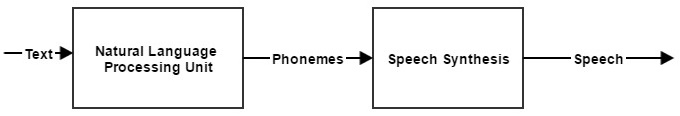
\includegraphics[width=\linewidth]{images/tts_bd.jpg}
  \caption{TTS Block Diagram}
  \label{fig:TTS Block Diagram}
\end{center}

In NLP unit, text is first converted into string of letters and then word boundaries are marked by
tokenizer. This is called normalization of text. Normalized data is then converted into phonetic strings
with the help of letter to sound rules after which Syllabifier marks syllable boundaries. Sound change
rules are applied on the syllabified date. Language modeling techniques are also applied for finding
context in which a specific word is used. As human has tendency to recognize basic rules for his native
language, it is easy to judge context of a word in a sentence and what should be correct pronunciation of
that word with respect to its context. For example, it can be guessed easily that “ ”پلin a sentence is used
for ( پلmoment) or ( پلbridge) for any native speaker of Urdu. Last stage of NLP is stress intonation
marker which adds stress and intonation to the text. Speech Synthesis unit converts symbolic information
received from NLP unit into audible speech with the help of different Digital Signal Processing
Techniques. The quality of speech synthesis system is detected by naturalness and intelligibility of the speech.

Partially blinded or fully blinded people usually suffer while using computer technology when there is no assistant or computer is not enough interactive. Due to which text to speech systems are becoming necessity of modern life. These systems increase the degree to which blind people can interact with sighted people \cite{klatt1987review} and could boost up their hope to survive in this world gracefully \cite{aida2010main}. Many applications of speech synthesis are emerging such as machines that read for blinds, aids for handicaps, computers that interact with user through speech. For all these applications a text to
speech that convert text to speech are used \cite{klatt1982klattalk}.


In digital world there are some people who can read and understand different languages and some
who can’t understand languages except their own languages. Speech to text conversion system can
also provide a facility to exchange information between people speaking different languages \cite{khilari2015review}. TTS systems are also needed to reduce the extinction of
minority languages. As minority languages of the world are facing challenge of extinction
considerable efforts are going on from last few years for their survival. Fon language is spoken in
Republic of Benin and some other regions of Africa and it is also facing challenge of extinction \cite{dagba2014text}.

Urdu is national language of Pakistan and it is spoken by more than 100 million people across the world \cite{top_30_languages}.
A Text-toSpeech (TTS) synthesis will be very helping for visually impaired, handicapped and illiterate people. These are the symbols which
collectively describe correct pronunciation of a word. This process is easy as compared to previous one
as number of such phonemes is limited for any language. For English, there are 44 such phonemes.
Similarly in Urdu, there are 44 consonants, 8 long vowels, 7 long nasal vowels, 3 short vowels and many
diphthongs \cite{saleem2002urdu}.

%
% Micro-optimization is a technique to reduce the overall operation count of
% floating point operations.  In a standard floating point unit, floating
% point operations are fairly high level, such as ``multiply'' and ``add'';
% in a micro floating point unit ($\mu$FPU), these have been broken down into
% their constituent low-level floating point operations on the mantissas and
% exponents of the floating point numbers.
%
% Chapter two describes the architecture of the $\mu$FPU unit, and the
% motivations for the design decisions made.
%
% Chapter three describes the design of the compiler, as well as how the
% optimizations discussed in section~\ref{ch1:opts} were implemented.
%
% Chapter four describes the purpose of test code that was compiled, and which
% statistics were gathered by running it through the simulator.  The purpose
% is to measure what effect the micro-optimizations had, compared to
% unoptimized code.  Possible future expansions to the project are also
% discussed.
%
% \section{Motivations for micro-optimization}
%
% The idea of micro-optimization is motivated by the recent trends in computer
% architecture towards low-level parallelism and small, pipelineable
% instruction sets \cite{patterson:risc,rad83}.  By getting rid of more
% complex instructions and concentrating on optimizing frequently used
% instructions, substantial increases in performance were realized.
%
% Another important motivation was the trend towards placing more of the
% burden of performance on the compiler.  Many of the new architectures depend
% on an intelligent, optimizing compiler in order to realize anywhere near
% their peak performance
% \cite{ellis:bulldog,pet87,coutant:precision-compilers}.  In these cases, the
% compiler not only is responsible for faithfully generating native code to
% match the source language, but also must be aware of instruction latencies,
% delayed branches, pipeline stages, and a multitude of other factors in order
% to generate fast code \cite{gib86}.
%
% Taking these ideas one step further, it seems that the floating point
% operations that are normally single, large instructions can be further broken
% down into smaller, simpler, faster instructions, with more control in the
% compiler and less in the hardware.  This is the idea behind a
% micro-optimizing FPU; break the floating point instructions down into their
% basic components and use a small, fast implementation, with a large part of
% the burden of hardware allocation and optimization shifted towards
% compile-time.
%
% Along with the hardware speedups possible by using a $\mu$FPU, there are
% also optimizations that the compiler can perform on the code that is
% generated.  In a normal sequence of floating point operations, there are
% many hidden redundancies that can be eliminated by allowing the compiler to
% control the floating point operations down to their lowest level.  These
% optimizations are described in detail in section~\ref{ch1:opts}.
%
% \section{Description of micro-optimization}\label{ch1:opts}
%
% In order to perform a sequence of floating point operations, a normal FPU
% performs many redundant internal shifts and normalizations in the process of
% performing a sequence of operations.  However, if a compiler can
% decompose the floating point operations it needs down to the lowest level,
% it then can optimize away many of these redundant operations.
%
% If there is some additional hardware support specifically for
% micro-optimization, there are additional optimizations that can be
% performed.  This hardware support entails extra ``guard bits'' on the
% standard floating point formats, to allow several unnormalized operations to
% be performed in a row without the loss information\footnote{A description of
% the floating point format used is shown in figures~\ref{exponent-format}
% and~\ref{mantissa-format}.}.  A discussion of the mathematics behind
% unnormalized arithmetic is in appendix~\ref{unnorm-math}.
%
% The optimizations that the compiler can perform fall into several categories:
%
% \subsection{Post Multiply Normalization}
%
% When more than two multiplications are performed in a row, the intermediate
% normalization of the results between multiplications can be eliminated.
% This is because with each multiplication, the mantissa can become
% denormalized by at most one bit.  If there are guard bits on the mantissas
% to prevent bits from ``falling off'' the end during multiplications, the
% normalization can be postponed until after a sequence of several
% multiplies\footnote{Using unnormalized numbers for math is not a new idea; a
% good example of it is the Control Data CDC 6600, designed by Seymour Cray.
% \cite{thornton:cdc6600} The CDC 6600 had all of its instructions performing
% unnormalized arithmetic, with a separate {\tt NORMALIZE} instruction.}.
%
% % This is an example of how you would use tgrind to include an example
% % of source code; it is commented out in this template since the code
% % example file does not exist.  To use it, you need to remove the '%' on the
% % beginning of the line, and insert your own information in the call.
% %
% %\tagrind[htbp]{code/pmn.s.tex}{Post Multiply Normalization}{opt:pmn}
%
% As you can see, the intermediate results can be multiplied together, with no
% need for intermediate normalizations due to the guard bit.  It is only at
% the end of the operation that the normalization must be performed, in order
% to get it into a format suitable for storing in memory\footnote{Note that
% for purposed of clarity, the pipeline delays were considered to be 0, and
% the branches were not delayed.}.
%
% \subsection{Block Exponent}
%
% In a unoptimized sequence of additions, the sequence of operations is as
% follows for each pair of numbers ($m_1$,$e_1$) and ($m_2$,$e_2$).
% \begin{enumerate}
%   \item Compare $e_1$ and $e_2$.
%   \item Shift the mantissa associated with the smaller exponent $|e_1-e_2|$
%         places to the right.
%   \item Add $m_1$ and $m_2$.
%   \item Find the first one in the resulting mantissa.
%   \item Shift the resulting mantissa so that normalized
%   \item Adjust the exponent accordingly.
% \end{enumerate}
%
% Out of 6 steps, only one is the actual addition, and the rest are involved
% in aligning the mantissas prior to the add, and then normalizing the result
% afterward.  In the block exponent optimization, the largest mantissa is
% found to start with, and all the mantissa's shifted before any additions
% take place.  Once the mantissas have been shifted, the additions can take
% place one after another\footnote{This requires that for n consecutive
% additions, there are $\log_{2}n$ high guard bits to prevent overflow.  In
% the $\mu$FPU, there are 3 guard bits, making up to 8 consecutive additions
% possible.}.  An example of the Block Exponent optimization on the expression
% X = A + B + C is given in figure~\ref{opt:be}.
%
% % This is an example of how you would use tgrind to include an example
% % of source code; it is commented out in this template since the code
% % example file does not exist.  To use it, you need to remove the '%' on the
% % beginning of the line, and insert your own information in the call.
% %
% %\tgrind[htbp]{code/be.s.tex}{Block Exponent}{opt:be}
%
% \section{Integer optimizations}
%
% As well as the floating point optimizations described above, there are
% also integer optimizations that can be used in the $\mu$FPU.  In concert
% with the floating point optimizations, these can provide a significant
% speedup.
%
% \subsection{Conversion to fixed point}
%
% Integer operations are much faster than floating point operations; if it is
% possible to replace floating point operations with fixed point operations,
% this would provide a significant increase in speed.
%
% This conversion can either take place automatically or or based on a
% specific request from the programmer.  To do this automatically, the
% compiler must either be very smart, or play fast and loose with the accuracy
% and precision of the programmer's variables.  To be ``smart'', the computer
% must track the ranges of all the floating point variables through the
% program, and then see if there are any potential candidates for conversion
% to floating point.  This technique is discussed further in
% section~\ref{range-tracking}, where it was implemented.
%
% The other way to do this is to rely on specific hints from the programmer
% that a certain value will only assume a specific range, and that only a
% specific precision is desired.  This is somewhat more taxing on the
% programmer, in that he has to know the ranges that his values will take at
% declaration time (something normally abstracted away), but it does provide
% the opportunity for fine-tuning already working code.
%
% Potential applications of this would be simulation programs, where the
% variable represents some physical quantity; the constraints of the physical
% system may provide bounds on the range the variable can take.
% \subsection{Small Constant Multiplications}
%
% One other class of optimizations that can be done is to replace
% multiplications by small integer constants into some combination of
% additions and shifts.  Addition and shifting can be significantly faster
% than multiplication.  This is done by using some combination of
% \begin{eqnarray*}
% a_i & = & a_j + a_k \\
% a_i & = & 2a_j + a_k \\
% a_i & = & 4a_j + a_k \\
% a_i & = & 8a_j + a_k \\
% a_i & = & a_j - a_k \\
% a_i & = & a_j \ll m \mbox{shift}
% \end{eqnarray*}
% instead of the multiplication.  For example, to multiply $s$ by 10 and store
% the result in $r$, you could use:
% \begin{eqnarray*}
% r & = & 4s + s\\
% r & = & r + r
% \end{eqnarray*}
% Or by 59:
% \begin{eqnarray*}
% t & = & 2s + s \\
% r & = & 2t + s \\
% r & = & 8r + t
% \end{eqnarray*}
% Similar combinations can be found for almost all of the smaller
% integers\footnote{This optimization is only an ``optimization'', of course,
% when the amount of time spent on the shifts and adds is less than the time
% that would be spent doing the multiplication.  Since the time costs of these
% operations are known to the compiler in order for it to do scheduling, it is
% easy for the compiler to determine when this optimization is worth using.}.
% \cite{magenheimer:precision}
%
% \section{Other optimizations}
%
% \subsection{Low-level parallelism}
%
% The current trend is towards duplicating hardware at the lowest level to
% provide parallelism\footnote{This can been seen in the i860; floating point
% additions and multiplications can proceed at the same time, and the RISC
% core be moving data in and out of the floating point registers and providing
% flow control at the same time the floating point units are active. \cite{byte:i860}}
%
% Conceptually, it is easy to take advantage to low-level parallelism in the
% instruction stream by simply adding more functional units to the $\mu$FPU,
% widening the instruction word to control them, and then scheduling as many
% operations to take place at one time as possible.
%
% However, simply adding more functional units can only be done so many times;
% there is only a limited amount of parallelism directly available in the
% instruction stream, and without it, much of the extra resources will go to
% waste.  One process used to make more instructions potentially schedulable
% at any given time is ``trace scheduling''.  This technique originated in the
% Bulldog compiler for the original VLIW machine, the ELI-512.
% \cite{ellis:bulldog,colwell:vliw}  In trace scheduling, code can be
% scheduled through many basic blocks at one time, following a single
% potential ``trace'' of program execution.  In this way, instructions that
% {\em might\/} be executed depending on a conditional branch further down in
% the instruction stream are scheduled, allowing an increase in the potential
% parallelism.  To account for the cases where the expected branch wasn't
% taken, correction code is inserted after the branches to undo the effects of
% any prematurely executed instructions.
%
% \subsection{Pipeline optimizations}
%
% In addition to having operations going on in parallel across functional
% units, it is also typical to have several operations in various stages of
% completion in each unit.  This pipelining allows the throughput of the
% functional units to be increased, with no increase in latency.
%
% There are several ways pipelined operations can be optimized.  On the
% hardware side, support can be added to allow data to be recirculated back
% into the beginning of the pipeline from the end, saving a trip through the
% registers.  On the software side, the compiler can utilize several tricks to
% try to fill up as many of the pipeline delay slots as possible, as
% seendescribed by Gibbons. \cite{gib86}
